\documentclass[border=4pt]{standalone}
\usepackage{amsmath,amssymb,amsfonts}
\usepackage{xcolor,colortbl,array,booktabs,multirow}
\usepackage{tikz}
\usetikzlibrary{arrows, automata, backgrounds, calendar, chains, decorations,
    matrix, mindmap, patterns, petri, positioning, shadows, shapes.geometric,
    trees, shapes, decorations.pathreplacing, calc, tikzmark, arrows.meta}
\newcommand{\st}{\text{ s.t. }}
\newcommand{\x}{\mathbf{x}}
\renewcommand{\b}{\mathbf{b}}
\newcommand{\A}{\mathbf{A}}
\newcommand{\R}{\mathbb{R}}
\newcommand{\RR}{\mathbb{R}}
\newcommand{\Z}{\mathbb{Z}}
\newcommand{\ZZ}{\mathbb{Z}}
\begin{document}
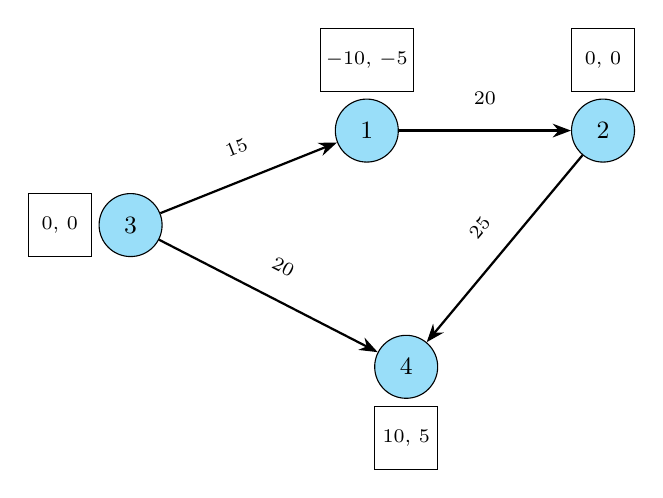
\begin{tikzpicture}[
    every node/.style={circle, draw=black, fill=cyan!40, minimum size=8mm, inner sep=1pt, font=\small},
    every edge/.style={draw, thick},
    >=Stealth,
    node distance=2.5cm and 3cm
  ]
  % Node positions match the networkx layout: 1 top-center, 2 top-right, 3 left, 4 bottom-center
  \node (n1) at (3,3) {1};
  \node (n2) at (6,3) {2};
  \node (n3) at (0,1.8) {3};
  \node (n4) at (3.5,0) {4};

  % Supply/demand annotations (commodity 1, commodity 2)
  \node[draw=black, fill=white, rectangle, font=\scriptsize, inner sep=2pt] at (3,3.9) {$-10,\,-5$};
  \node[draw=black, fill=white, rectangle, font=\scriptsize, inner sep=2pt] at (6,3.9) {$0,\,0$};
  \node[draw=black, fill=white, rectangle, font=\scriptsize, inner sep=2pt] at (-0.9,1.8) {$0,\,0$};
  \node[draw=black, fill=white, rectangle, font=\scriptsize, inner sep=2pt] at (3.5,-0.9) {$10,\,5$};

  % Arcs with shared capacities
  \draw[->, thick] (n3) -- (n1) node[midway, sloped, above, font=\scriptsize, fill=none, draw=none, rectangle] {15};
  \draw[->, thick] (n1) -- (n2) node[midway, above, font=\scriptsize, fill=none, draw=none, rectangle] {20};
  \draw[->, thick] (n2) -- (n4) node[midway, sloped, above, font=\scriptsize, fill=none, draw=none, rectangle] {25};
  \draw[->, thick] (n3) -- (n4) node[midway, sloped, above, font=\scriptsize, fill=none, draw=none, rectangle] {20};
\end{tikzpicture}
\end{document}
